\documentclass[tikz,border=2pt]{standalone}
\usepackage{amsmath,amssymb}
\usepackage{pgfplots}
\pgfplotsset{compat=1.18}

\begin{document}
% Symmetric about a: the density is its own mirror image in the line x = a, so X - a and
% a - X have the same distribution and (when it exists) the mean equals a.
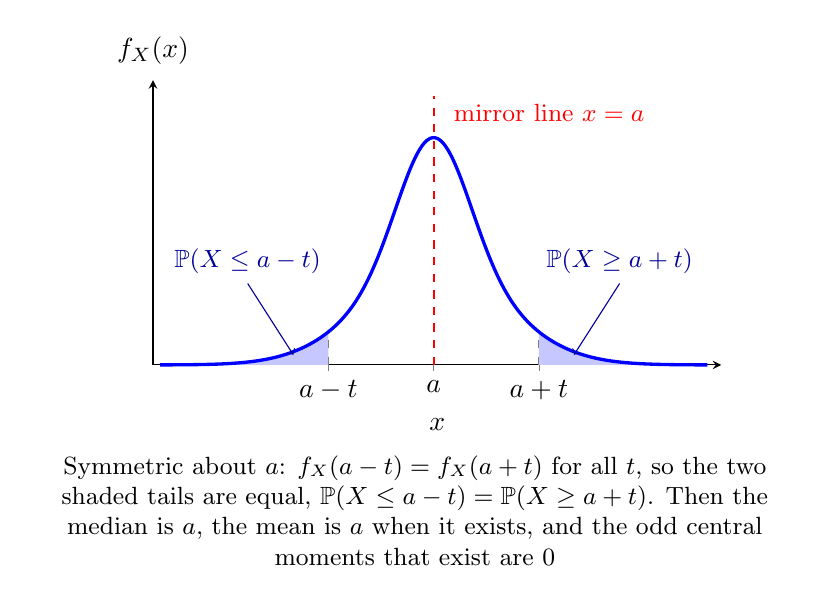
\begin{tikzpicture}
	\begin{axis}[
		axis lines=left, xmin=-1, xmax=7.1, ymin=0, ymax=0.7,
		xtick={1.5,3,4.5}, xticklabels={$a-t$,$a$,$a+t$}, ytick=\empty,
		xlabel={$x$}, ylabel={$f_X(x)$}, ylabel style={rotate=-90, anchor=south, at={(axis description cs:0,1.02)}},
		samples=200, smooth, width=8.8cm, height=5.2cm, clip=false
		]
		\addplot[fill=blue!22, draw=none, domain=4.5:6.9] {0.6*exp(-(x-3)^2/2)/sqrt(2*pi)+0.4*exp(-(x-3)^2/0.5)/sqrt(0.5*pi)} \closedcycle;
		\addplot[fill=blue!22, draw=none, domain=-0.9:1.5] {0.6*exp(-(x-3)^2/2)/sqrt(2*pi)+0.4*exp(-(x-3)^2/0.5)/sqrt(0.5*pi)} \closedcycle;
		\addplot[blue, very thick, domain=-0.9:6.9] {0.6*exp(-(x-3)^2/2)/sqrt(2*pi)+0.4*exp(-(x-3)^2/0.5)/sqrt(0.5*pi)};
		\draw[red, dashed, thick] (axis cs:3,0) -- (axis cs:3,0.66);
		\draw[gray, dashed] (axis cs:1.5,0) -- (axis cs:1.5,0.081);
		\draw[gray, dashed] (axis cs:4.5,0) -- (axis cs:4.5,0.081);
		\node[blue!60!black, font=\small, anchor=south] at (axis cs:0.35,0.2) {$\mathbb{P}(X\le a-t)$};
		\draw[blue!60!black, ->] (axis cs:0.35,0.2) -- (axis cs:1.0,0.025);
		\node[blue!60!black, font=\small, anchor=south] at (axis cs:5.65,0.2) {$\mathbb{P}(X\ge a+t)$};
		\draw[blue!60!black, ->] (axis cs:5.65,0.2) -- (axis cs:5.0,0.025);
		\node[red, anchor=west, font=\small] at (axis cs:3.15,0.62) {mirror line $x=a$};
	\end{axis}
	\node[anchor=north, font=\small, align=flush center, text width=9.6cm] at ([yshift=-2pt]current axis.outer south) {Symmetric about $a$: $f_X(a-t)=f_X(a+t)$ for all $t$, so the two shaded tails are equal, $\mathbb{P}(X\le a-t)=\mathbb{P}(X\ge a+t)$. Then the median is $a$, the mean is $a$ when it exists, and the odd central moments that exist are $0$};
\end{tikzpicture}
\end{document}
